\documentclass[10pt,pdf,hyperref={unicode}]{beamer}

\mode<presentation>
{
    \usetheme{boxes}
    \beamertemplatenavigationsymbolsempty
    \setbeamertemplate{footline}[page number]
    \usecolortheme{seagull}
    \setbeamersize{text margin left=0.7em, text margin right=0.7em}
}

\usepackage[T2A]{fontenc}
\usepackage[utf8]{inputenc}
\usepackage[english,russian]{babel}
\usepackage{amsmath}
\usepackage{amssymb}
\usepackage{bm}
\usepackage{booktabs}
\usepackage{graphicx}
\usepackage{indentfirst}
\usepackage{ragged2e}
\usepackage{subfig}

\graphicspath{{../paper/thesis_assets/figures/}}

\newtheorem{rustheorem}{Теорема}
\newcommand{\R}{\mathbb{R}}
\newcommand{\E}{\mathbb{E}}
\newcommand{\cX}{\mathcal{X}}
\newcommand{\norm}[1]{\left\|#1\right\|}
\newcommand{\inner}[2]{\left\langle #1,#2 \right\rangle}
\newcommand{\argmin}{\operatorname*{arg\,min}}

\newcommand{\PresentationTitle}{Приложения алгоритма Франк-Вульфа к задачам машинного обучения}
\newcommand{\PresentationShortTitle}{Frank--Wolfe в ML}
\newcommand{\PresentationAuthor}{Игнашин Игорь Николаевич}
\newcommand{\PresentationInstitute}{Московский физико-технический институт}
\newcommand{\PresentationProgram}{09.04.01 Информатика и вычислительная техника}
\newcommand{\PresentationSupervisor}{Научный руководитель: д.ф.-м.н. Грабовой А. О.}
\newcommand{\PresentationPlaceDate}{Москва, 2026}

\title[\PresentationShortTitle]{\PresentationTitle}
\author{\large \PresentationAuthor}
\institute{\large
\PresentationInstitute\\
~\\
\footnotesize{\PresentationProgram\\
~\\
\PresentationSupervisor}
}
\date{\footnotesize{\PresentationPlaceDate}}

\begin{document}

\begin{frame}
    \titlepage
\end{frame}

\begin{frame}{Почему Frank--Wolfe}
\justifying
Во многих задачах машинного обучения и сетевой оптимизации требуется решать
\[
    \min_{x\in\cX} f(x),
\]
где множество $\cX$ имеет простую линейную оптимизацию, но дорогую евклидову проекцию.

\bigskip

\begin{block}{Идея метода условного градиента}
На каждой итерации вместо проекции решается линейная подзадача
\[
    s_k\in\argmin_{s\in\cX}\inner{\nabla f(x_k)}{s},
    \qquad
    x_{k+1}=x_k+\gamma_k(s_k-x_k).
\]
\end{block}

\vspace{0.2cm}
Это делает Frank--Wolfe естественным инструментом для $l_1$-ограничений, симплексов,
транспортных политопов и блочных произведений множеств.
\end{frame}

\begin{frame}{Главное ограничение базового FW}
\justifying
Классический Frank--Wolfe проекционно-свободен, но не решает все вычислительные проблемы.

\bigskip

\begin{columns}[T]
\begin{column}{0.32\textwidth}
\textbf{Направление}\\
Зигзагообразность траектории около границы допустимого множества.
\end{column}
\begin{column}{0.32\textwidth}
\textbf{Оракул}\\
Полный линейный оракул может быть дорогим на крупных блочных задачах.
\end{column}
\begin{column}{0.32\textwidth}
\textbf{Данные}\\
Функция и данные могут быть распределены между агентами сети.
\end{column}
\end{columns}

\bigskip

\begin{block}{Линия работы}
Модификации FW рассматриваются как способы ускорить разные части одной итерации:
выбор направления, вызов линейного оракула и коммуникацию.
\end{block}
\end{frame}

\begin{frame}{Структура результатов}
\justifying
В работе объединены четыре связанных направления.

\begin{enumerate}
    \item Модификации FW с памятью о предыдущих направлениях в транспортной задаче.
    \item Перенос CFW и NFW на гладкие задачи машинного обучения.
    \item Стохастический блочно-координатный FW для транспортных сетей.
    \item Децентрализованный блочно-координатный FW для распределенной оптимизации.
\end{enumerate}

\bigskip

\begin{center}
\begin{tabular}{lll}
\toprule
Узкое место & Метод & Результат \\
\midrule
направление & CFW/NFW & гарантия по FW-зазору \\
полный LMO & SOFW/BCFW & $O(1/k)$ в ожидании \\
коммуникации + LMO & DBCFW & $O(1/t)$ для $x_{\mathrm{avg},t}$ \\
\bottomrule
\end{tabular}
\end{center}
\end{frame}

\begin{frame}{Цель и задачи}
\justifying
\textbf{Цель:} развить и теоретически обосновать модификации Frank--Wolfe для задач,
где стоимость линейного оракула, выбора направления или коммуникации определяет
практическую эффективность метода.

\bigskip

\textbf{Задачи:}
\begin{enumerate}
    \item Сформулировать CFW/NFW для гладкой выпуклой задачи на компактном множестве.
    \item Получить оценку сходимости CFW по зазору Frank--Wolfe.
    \item Описать SOFW как стохастический блочно-координатный FW и вывести оценку в ожидании.
    \item Сформулировать DBCFW и доказать оценку сходимости для средней точки сети.
    \item Проверить практический эффект на ML-задачах и транспортных сетях.
\end{enumerate}
\end{frame}

\begin{frame}{CFW и NFW: память о направлениях}
\justifying
В CFW новое направление строится как комбинация текущего FW-направления и предыдущего направления:
\[
    d_k
    =
    \alpha d_k^{FW}
    +
    (1-\alpha)(1-\gamma_{k-1})d_{k-1}.
\]

\bigskip

\begin{block}{Что это дает}
\begin{itemize}
    \item направление учитывает локальную геометрию траектории;
    \item NFW обобщает эту идею на несколько прошлых направлений;
    \item для ML-задач произведение на гессиан заменяется конечными разностями градиентов.
\end{itemize}
\end{block}

\[
    \nabla^2 f(x_k)d_{k-1}
    \approx
    \nabla f(x_k)-\nabla f(x_{k-1}).
\]
\end{frame}

\begin{frame}{Теоретический результат для CFW}
\justifying
Пусть $\cX$ выпукло и компактно, а $f$ выпукла и имеет $L$-липшицев градиент на $\cX$.
FW-зазор:
\[
    g_k=\inner{\nabla f(x_k)}{x_k-s_k^{FW}}.
\]

\begin{rustheorem}
Для CFW с параметром $\alpha_0\in(0,1]$ и точным линейным поиском
\[
    g_N^\ast=\min_{1\leq k\leq N}g_k
    \leq
    \frac{\max\{2h_0,LR^2\}}{\alpha_0\sqrt{N+1}}.
\]
\end{rustheorem}

\vspace{0.15cm}
Итог: CFW сохраняет стандартный порядок сходимости по зазору, но может улучшать
практическое направление шага.
\end{frame}

\begin{frame}{Эксперименты в машинном обучении}
\justifying
Рассматривалась логистическая регрессия с ограничением на $l_1$-норму.
Сравнивались FW, FW с линейным поиском, CFW и NFW.

\bigskip

\begin{center}
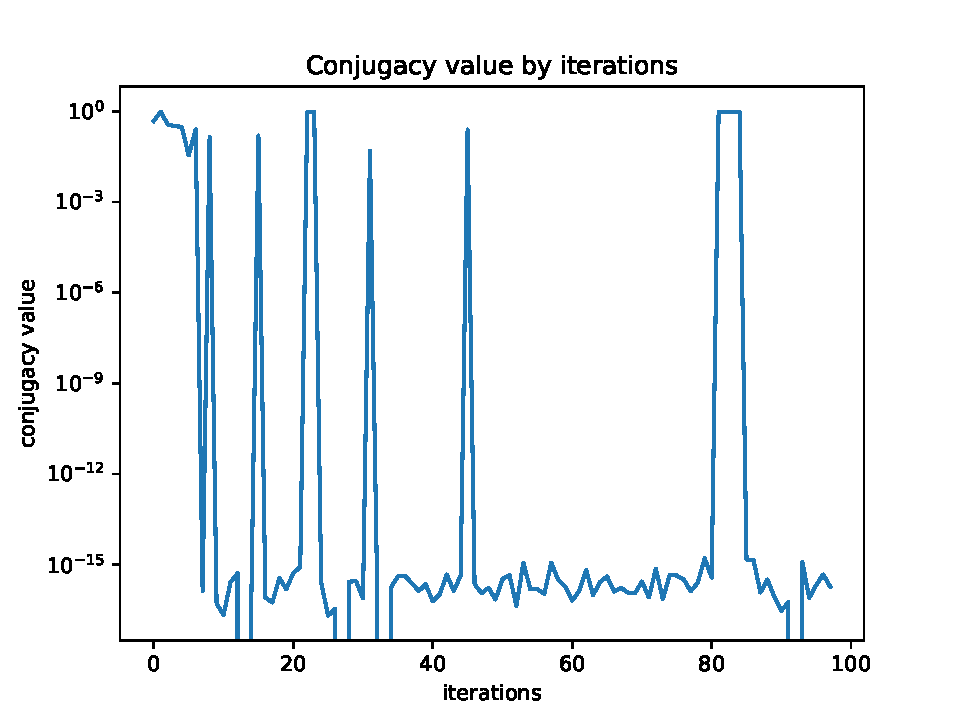
\includegraphics[height=0.50\textheight,keepaspectratio]{cfw_ml/Experiment_3_fig_1.pdf}
\end{center}

\vspace{-0.15cm}
\footnotesize
CFW/NFW особенно полезны, когда активное ограничение создает зигзагообразное поведение базового FW.
\end{frame}

\begin{frame}{SOFW: блочный оракул для транспортных сетей}
\justifying
В модели Бекмана допустимое множество имеет блочную структуру по OD-парам или источникам.
Полная итерация FW требует решать задачи кратчайших путей для всех источников.

\[
    \mathcal{C}_{FW}
    =
    \mathcal{O}\bigl(n(E+V\log V)\bigr).
\]

\begin{block}{Stochastic Origin Frank--Wolfe}
На каждой итерации выбирается только часть блоков, и линейный оракул решается
для выбранных источников:
\[
    \mathcal{C}_{SOFW}
    =
    \mathcal{O}\bigl(\alpha n(E+V\log V)\bigr).
\]
\end{block}

Цена ускорения: нужно хранить разложение потока по источникам и учитывать
дисперсию стохастического направления.
\end{frame}

\begin{frame}{Теоретический результат для SOFW}
\justifying
Для батчевого SOFW направление строится по случайному подмножеству блоков $\mathcal{I}_k$:
\[
    d_k=\frac{1}{m}\sum_{w\in\mathcal{I}_k}(s_k^{[w]}-x_k^{[w]}).
\]

\begin{rustheorem}
При шаге
\[
    \gamma_k=\frac{2|OD|}{k+2|OD|}
\]
выполнена оценка
\[
    \E[\Psi(F(x_k))]-\Psi(F(x^\ast))
    \leq
    \frac{2|OD|}{k+2|OD|}
    \left(C_\Psi^\otimes+\Psi(F(x_0))-\Psi(F(x^\ast))\right).
\]
\end{rustheorem}

Итог: стохастизация уменьшает стоимость итерации, не меняя порядок гарантии.
\end{frame}

\begin{frame}{SOFW: вычислительный эффект}
\justifying
Эксперименты проводились на транспортных сетях из открытого репозитория
TransportationNetworks. Сравнивались FW, SOFW и взвешенный SOFW-w.

\begin{center}
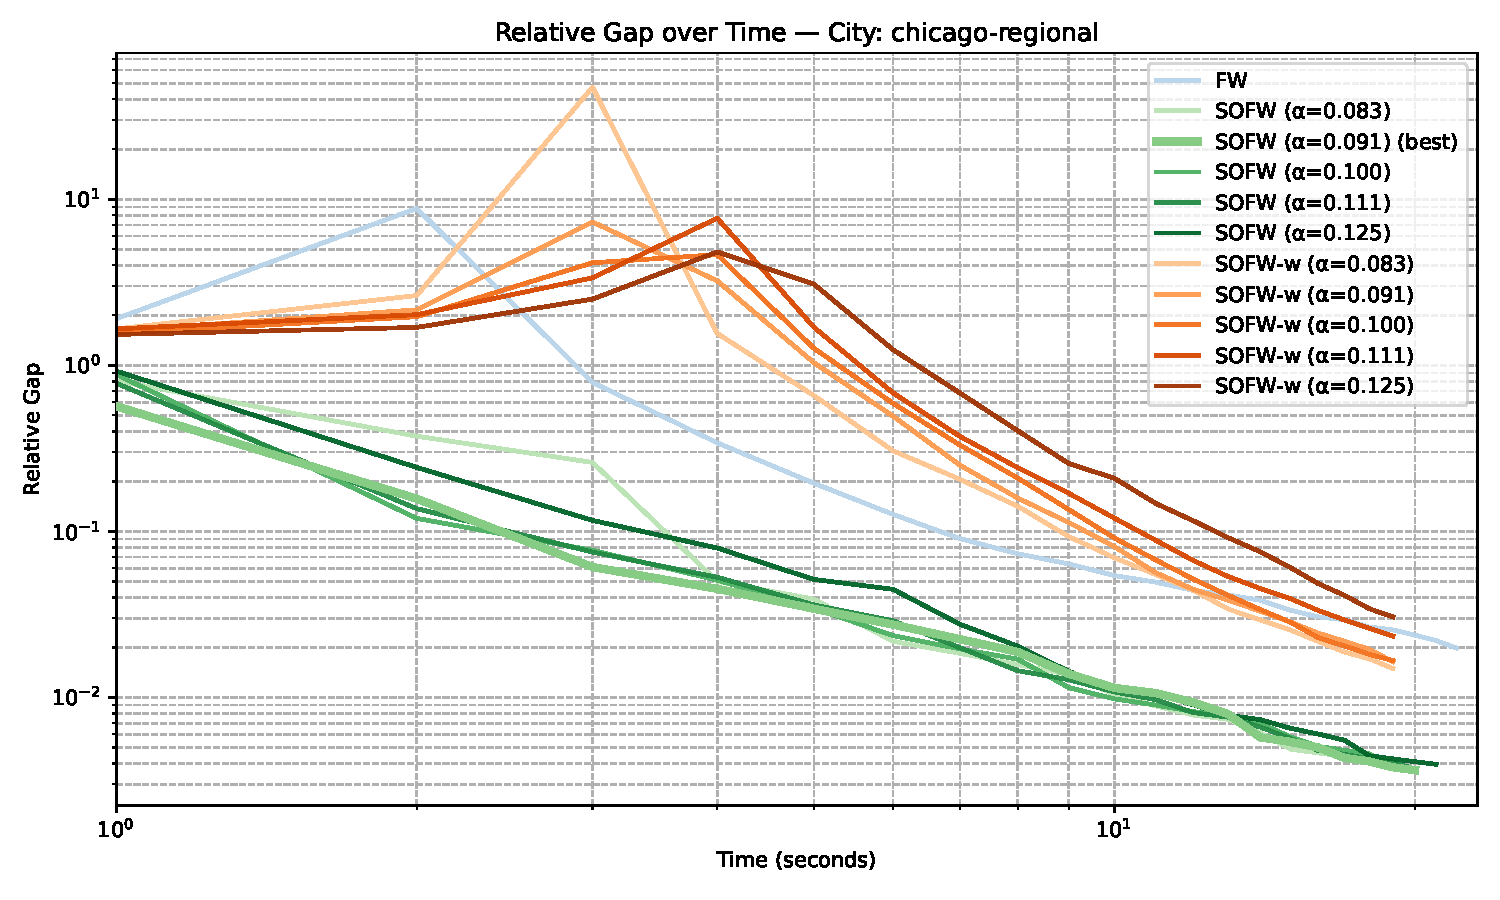
\includegraphics[height=0.56\textheight,keepaspectratio]{scfw/chicago-regional.pdf}
\end{center}

\vspace{-0.1cm}
\footnotesize
На крупных сетях стохастический оракул быстрее уменьшает относительный зазор
при одинаковом вычислительном бюджете.
\end{frame}

\begin{frame}{DBCFW: распределенная постановка}
\justifying
Пусть есть $N$ агентов, и агент $i$ знает только локальную функцию $f_i$:
\[
    \min_{x\in D} f(x),
    \qquad
    f(x)=\frac{1}{N}\sum_{i=1}^{N} f_i(x),
    \qquad
    D=D_1\times\dots\times D_n.
\]

\begin{columns}[T]
\begin{column}{0.48\textwidth}
\textbf{Децентрализация}
\begin{itemize}
    \item локальная копия $x_t^i$;
    \item обмен только с соседями;
    \item матрица смешивания $W_t$.
\end{itemize}
\end{column}
\begin{column}{0.48\textwidth}
\textbf{Блочность}
\begin{itemize}
    \item выбирается батч блоков $I_t^i$;
    \item LMO решается на $D_t^i$;
    \item стоимость зависит от размера батча.
\end{itemize}
\end{column}
\end{columns}
\end{frame}

\begin{frame}{Алгоритм DBCFW}
\justifying
На каждой итерации агент выполняет три шага.

\begin{enumerate}
    \item \textbf{Консенсус по точкам}
    \[
        \tilde x_t^i=\sum_j (W_t)_{ij}x_t^j.
    \]
    \item \textbf{Отслеживание градиента}
    \[
        g_t^i=\tilde g_{t-1}^i+\nabla f_i(\tilde x_t^i)-\nabla f_i(\tilde x_{t-1}^i),
        \qquad
        \tilde g_t^i=\sum_j(W_t)_{ij}g_t^j.
    \]
    \item \textbf{Блочный линейный оракул}
    \[
        v_t^i\in\argmin_{v\in D_t^i}\inner{\tilde g_t^i}{v},
        \qquad
        x_{t+1}^i=(1-\gamma_t)\tilde x_t^i+\gamma_t v_t^i.
    \]
\end{enumerate}
\end{frame}

\begin{frame}{Теоретический результат для DBCFW}
\justifying
При стандартных предположениях о гладкости, выпуклости, компактности $D$ и
сжатии коммуникационной ошибки получена рекурсия для средней точки сети:
\[
    h_t=\E[f(x_{\mathrm{avg},t})-f(x^\ast)].
\]

\begin{rustheorem}
При шаге
\[
    \gamma_t=\frac{2n}{B(t+\tau)},\qquad \tau=\frac{2n}{B},
\]
выполнено
\[
    h_t\leq \frac{\widetilde A_\tau}{t+\tau},
    \qquad
    \E[f(x_{\mathrm{avg},t})-f(x^\ast)]=O(1/t).
\]
\end{rustheorem}

Влияние консенсуса, gradient tracking и размера батча входит в константу,
но не ухудшает порядок сходимости.
\end{frame}

\begin{frame}{Основные результаты и публикации}
\justifying
\begin{columns}[T]
\begin{column}{0.58\textwidth}
\textbf{Результаты}
\begin{enumerate}
    \item CFW/NFW перенесены на ML без явного гессиана.
    \item Для CFW доказано $g_N^\ast=O(N^{-1/2})$.
    \item Для SOFW получено $O(1/k)$ в ожидании.
    \item Для DBCFW доказано
    $\E[f(x_{\mathrm{avg},t})-f(x^\ast)]=O(1/t)$.
    \item Эксперименты подтверждают выигрыш CFW/NFW и SOFW.
\end{enumerate}
\end{column}
\begin{column}{0.38\textwidth}
\textbf{Публикации}
\begin{itemize}
    \item КИМ, 2024: модификации FW для транспортных потоков.
    \item Journal of Mathematical Sciences, 2025: SOFW для traffic assignment.
\end{itemize}

\vspace{0.2cm}
\textbf{Дальше}
\begin{itemize}
    \item DBCFW на распределенных ML-задачах;
    \item блочные кривизны в константах;
    \item NFW + стохастические блоки.
\end{itemize}
\end{column}
\end{columns}
\end{frame}

\end{document}
